% Created by Takeuchi on Feb. 2020
\documentclass[dvipdfmx, 11pt,]{beamer}

%%%% Packages %%%%%
%\usepackage{bxdpx-beamer}
%\usepackage{minijs}
%\usepackage{otf}
%\usepackage{tabularx}
%\usepackage{graphicx}
% \usepackage{graphicx}
% \usepackage{amsmath,amssymb,amsthm}
% \usepackage{multirow}
\usepackage{multicol}
% \usepackage{url}
\usepackage{colortbl}
\usepackage{tikz}
\usetikzlibrary{arrows,shapes,calc,intersections}
\usetikzlibrary{positioning}
\usetikzlibrary{fit}
% \usepackage{alltt}
% \usepackage{bm}
\usepackage{listings,jlisting}
% \lstset{
%   basicstyle={\ttfamily\tiny},
%   tabsize=2,
%   breaklines=true,
%   %numbers=left,
%}
% captionpos=b,frame=single,
% columns=fullflexible,keepspaces=true,%

% \usepackage{listings}

\lstset{
 basicstyle=\ttfamily\tiny\color{black},
 keepspaces=true,
 escapechar=|,
 columns=[l]{fullflexible},
 commentstyle={\color{red}},
 stringstyle={\color{blue}},
 % literrate =%
 %   {:-}{{\textcolor{black}{:-}}}2%
 %   {,}{{\textcolor{black}{,}}}1%
 %   {.}{{\textcolor{black}{.}}}1%
}
%%%% Fonts %%%%%
\renewcommand{\kanjifamilydefault}{\gtdefault}
% \usepackage{otf} % otfパッケージ
\usepackage[deluxe]{otf} 
\usepackage{txfonts} % 数式・英文ローマン体を Lxfont にする
% \usepackage[T1]{fontenc} % 8bit フォント
% \usepackage{minijs}
% \usepackage{textcomp} % 欧文フォントの追加
% \usepackage[utf8]{inputenc} % 文字コードをUTF-8

%%%%% Beamer %%%%%
\usetheme{Madrid}
\useinnertheme{rectangles}
%\useoutertheme{smoothbars}
\setbeamercolor{enumerate}{fg=white, bg=black}
\usefonttheme{professionalfonts}
\setbeamertemplate{frametitle}[default][center]
\setbeamertemplate{navigation symbols}{}
% \setbeamercovered{transparent} % 好みに応じてどうぞ
\setbeamertemplate{footline}[frame number]
\setbeamercolor{page number in head/foot}{fg=black} % ページ数を表示する
% \setbeamerfont{footline}{size=\normalsize,series=\bfseries}
\setbeamerfont{footline}{size=\scriptsize,series=\mdseries}
\setbeamercolor{footline}{fg=black,bg=black}
\setbeamertemplate{blocks}[rounded][shadow=true]
\setbeamertemplate{items}[ball]
% \setbeamertemplate{enumerate items}[default]
% \setbeamerfont{alerted text}{series=\bfseries}

%%%% My macro %%%%%
%%%%%%%%%%%%%%%%%%%%%%%%%%%%%%%%%%%%%%%%%%%%%%%%%%%%%%%%%%%%%%%%
% User-defined Macro
%%%%%%%%%%%%%%%%%%%%%%%%%%%%%%%%%%%%%%%%%%%%%%%%%%%%%%%%%%%%%%%%
\newcommand{\compress}{\itemsep0pt\parsep0pt\parskip0pt\partopsep0pt}
% \newcommand{\compress}{\itemsep1pt plus1pt\parsep0pt\parskip0pt}
% \newcommand{\code}[1]{\lstinline[basicstyle=\ttfamily]{#1}}
\newcommand{\gringo}{\textit{gringo}}
\newcommand{\clasp}{\textit{clasp}}
\newcommand{\clingo}{\textit{clingo}}
\newcommand{\teaspoon}{\textit{teaspoon}}
\newcommand{\sat}{\textsf{SAT}}
\newcommand{\unsat}{\textsf{UNSAT}}
% \newcommand{\web}[2]{\href{#1}{#2\ \raisebox{-0.15ex}{\beamergotobutton{Web}}}}
% \newcommand{\doi}[2]{\href{#1}{#2\ \raisebox{-0.15ex}{\beamergotobutton{DOI}}}}
% \newcommand{\weblink}[1]{\web{#1}{#1}}
% \newcommand{\imp}{\mathrel{\Rightarrow}}
% \newcommand{\Iff}{\mathrel{\Leftrightarrow}}
% \newcommand{\mybox}[1]{\fbox{\rule[.2cm]{0cm}{0cm}\mbox{${#1}$}}}
% \newcommand{\mycbox}[2]{\tikz[baseline]\node[fill=#1!10,anchor=base,rounded corners=2pt] () {#2};}
% \newcommand{\naf}[1]{\ensuremath{{\sim\!\!{#1}}}}
% \newcommand{\head}[1]{\ensuremath{\mathit{head}(#1)}}
% \newcommand{\body}[1]{\ensuremath{\mathit{body}(#1)}}
% \newcommand{\atom}[1]{\ensuremath{\mathit{atom}(#1)}}
% \newcommand{\poslits}[1]{\ensuremath{{#1}^+}}
% \newcommand{\neglits}[1]{\ensuremath{{#1}^-}}
% \newcommand{\pbody}[1]{\poslits{\body{#1}}}
% \newcommand{\nbody}[1]{\neglits{\body{#1}}}
% \newcommand{\Cn}[1]{\ensuremath{\mathit{Cn}(#1)}}
% \newcommand{\reduct}[2]{\ensuremath{#1^{#2}}}
% \newcommand{\OK}{\mbox{\textcolor{green}{\Pisymbol{pzd}{52}}}}
% \newcommand{\KO}{\mbox{\textcolor{red}{\Pisymbol{pzd}{56}}}}
% \newcommand{\code}[1]{\lstinline[basicstyle=\ttfamily]{#1}}
% \newcommand{\lw}[1]{\smash{\lower2.ex\hbox{#1}}}
\newcommand{\llw}[1]{\smash{\lower3.ex\hbox{#1}}}

\newenvironment{tableC}{%
  \scriptsize
  \renewcommand{\arraystretch}{0.9}
  \tabcolsep = 0.6mm
  % \begin{tabular}[t]{p{6mm}|rlr|rlr|rlr|rlr|rlr}\hline
  %   \multicolumn{1}{l|}{\llw{問題   }} &
  \begin{tabular}[t]{l|rlr|rlr|rlr|rlr|rlr}\hline
    \multicolumn{1}{l|}{\llw{問題}} &
    \multicolumn{3}{c|}{UD1} &
    \multicolumn{3}{c|}{UD2} &
    \multicolumn{3}{c|}{UD3} &
    \multicolumn{3}{c|}{UD4} &
    \multicolumn{3}{c}{UD5} \\
    & 
    \multicolumn{1}{c}{既知の} & & \multicolumn{1}{c|}{ASP} & 
    \multicolumn{1}{c}{既知の} & & \multicolumn{1}{c|}{ASP} & 
    \multicolumn{1}{c}{既知の} & & \multicolumn{1}{c|}{ASP} & 
    \multicolumn{1}{c}{既知の} & & \multicolumn{1}{c|}{ASP} & 
    \multicolumn{1}{c}{既知の} & & \multicolumn{1}{c}{ASP} \\
    & 
    ベスト & &  & 
    ベスト & &  & 
    ベスト & &  & 
    ベスト & &  & 
    ベスト & &  \\
    \hline
  }{%
    \hline
  \end{tabular}
}

\newcommand{\nodeVP}[3]{
  \coordinate[#2] (#1);
  \draw[fill=cyan!30] (#1)--+(-1,0)--+(0,1)--+(1,0)--cycle;
  \draw (#1)node[above]{\tiny{#3}};
  \draw[fill=black] (#1) +(-0.5,0.5)--+(0.5,0.5)--+(0,1)--cycle;
  \node[rectangle,above=0.5cm of #1,white](vp){\tiny{VP}};
  \coordinate[below=0.5cm of #1] (via_#1);
  \draw (via_#1)node[above right]{\tiny{[1..1]}};
  \draw (via_#1) +(170:0.2) arc (170:370:0.2);
  \draw (#1)--(via_#1);

}
\newcommand{\nodeTrans}[3]{
  \coordinate[#2] (#1);
  \draw[fill=cyan!30] (#1)--+(-1,0)--+(0,1)--+(1,0)--cycle;
  \draw (#1)node[above]{\tiny{#3}};
  \draw[fill=black] (#1) +(-0.5,0.5)--+(0.5,0.5)--+(0,1)--cycle;
  \node[rectangle,above=0.5cm of #1,white](vp){\tiny{VP}};
  \coordinate[below=1.7cm of #1] (via_#1);
  \draw (via_#1)node[below=0.2cm]{\tiny{[1..1]}};
  \draw (via_#1) +(135:0.2) arc (135:405:0.2);
  \draw (#1)--(via_#1);

}

\newcommand{\nodeVPdashed}[3]{
  \coordinate[#2] (#1);
  \draw[fill=cyan!30,dashed] (#1)--+(-1,0)--+(0,1)--+(1,0)--cycle;
  \draw (#1)node[above]{\tiny{#3}};
  \fill[black] (#1) +(-0.5,0.5)--+(0.5,0.5)-- +(0,1)--cycle;
  \node[rectangle,above=0.5cm of #1,white](vp){\tiny{VP}};
  \coordinate[below=0.5cm of #1] (via_#1);
  \draw (via_#1)node[above right]{\tiny{[1..1]}};
  \draw (via_#1) +(-0.2,0) arc (180:360:0.2);
  \draw (#1)--(via_#1);

}

\newcommand{\nodeV}[4]{
  \node [draw,inner xsep=2pt,#2,fill=black!10,font=\tiny] (#1){
      \begin{tabular}{l}
       #3\\
       #4\\
      \end{tabular}
  };
  \fill [black] (#1.north west)--++(0,-2mm)--++(1mm,0)--++(1mm,0)--++(0,2mm); 
  \draw (#1.north west) ++(1mm,-1mm) node[white]{\tiny{v}};
}

\newcommand{\nodeVchoiced}[4]{
  \node [draw,inner xsep=2pt,#2,fill=red!50,font=\tiny] (#1){
      \begin{tabular}{l}
       #3\\
       #4\\
      \end{tabular}
  };
  \fill [black] (#1.north west)--++(0,-2mm)--++(1mm,0)--++(1mm,0)--++(0,2mm); 
  \draw (#1.north west) ++(1mm,-1mm) node[white]{\tiny{v}};

}


%%%%%%%%%%%%%%%%%%%%%%%%%%%%%%%%%%%%%%%%%%%%%%%%%%%%
\title{車両装備仕様問題に対する\\解集合プログラミングの適用}
\author{竹内 頼人(名古屋大学情報学研究科) \and \\ 番原 睦則(名古屋大学情報学研究科)}
%\institute{番原研究室}
\date{2020年7月X日}
\begin{document}
\begin{frame}
 \titlepage
\end{frame}
%%%%%%%%%%%%%%%%%%%%%%%%%%%%%%%%%%%%%%%%%%%%%%%%%%%%
\begin{frame}{車両装備仕様問題}
  \begin{itemize}
  \item 車両の装備を決定するには,販売される国や地域の法規や規制,
    地域や市場の特性,市場の嗜好や競合など十分に考慮する必要がある.
  \item 現状では専門知識をもつ技術者の多大な労力が費やされている.
  \item 日本では2020年度から,
    \structure{\bf 企業別平均燃費}
    (Corporate Average Fuel Efficiency; \structure{\bf CAFE})基準
    と呼ばれる燃費規制が採用されている.
  \end{itemize}
  \vfill
  \begin{alertblock}{車両装備仕様問題}
    \begin{itemize}
    \item 組合せ最適化問題として定式化される.
    \item \alert{個数制約},\alert{要求・排他制約},\alert{燃費制約}(CAFE基準)から構成される.
    \item \alert{販売台数を最大化}する\textbf{装備仕様}
      (装備タイプと装備オプションの組合せ)を求めることが目的である.
    \end{itemize}
  \end{alertblock}
 \begin{itemize}
  \item 本研究ではCAFE基準に基づく車両装備仕様問題(CAFE問題)を対象とする.
 \end{itemize}
\end{frame}
%%%%%%%%%%%%%%%%%%%%%%%%%%%%%%%%%%%%%%%%%%%%%%%%%%%%
\begin{frame}{CAFE問題の例}
  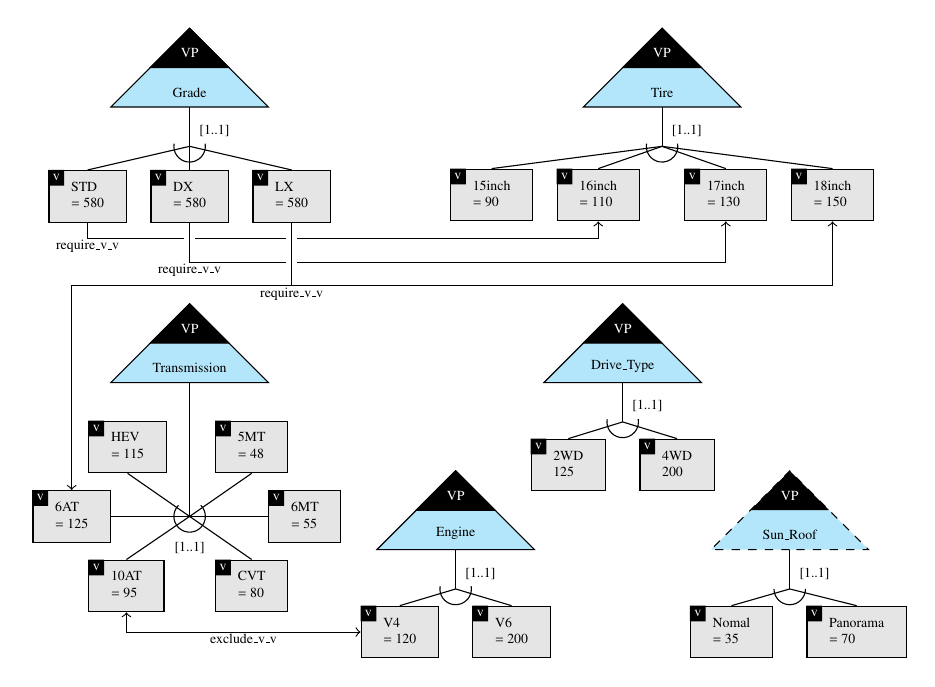
\begin{tikzpicture}
 % Grade
  \nodeVP{grade}{at={(0,0)}}{Grade};
  \nodeV{dx}{below=0.3cm of via_grade}{DX}{= 580};
  \draw(via_grade)--(dx.north);
  \nodeV{std}{left=0.3cm of dx}{STD}{= 580};
  \draw(via_grade)--(std.north);
  \nodeV{lx}{right=0.3cm of dx}{LX}{= 580};
  \draw(via_grade)--(lx.north);

  % Tire
  \nodeVP{tire}{right=6cm of grade}{Tire};
  \nodeV{16inch}{below left=0.4cm of via_tire}{16inch}{= 110};
  \nodeV{17inch}{below right=0.4cm of via_tire}{17inch}{= 130};
  \nodeV{15inch}{left=0.3cm of 16inch}{15inch}{= 90};
  \nodeV{18inch}{right=0.3cm of 17inch}{18inch}{= 150};
  \draw (via_tire)--(15inch.north);
  \draw (via_tire)--(16inch.north);
  \draw (via_tire)--(17inch.north);
  \draw (via_tire)--(18inch.north);

  % Transmission
  \nodeTrans{trans}{below=3.5cm of grade}{Transmission};
  \nodeV{6at}{left=1cm of via_trans}{6AT}{= 125};
  \nodeV{hev}{above right=0.3cm of 6at.north}{HEV}{= 115};
  \nodeV{10at}{below right=0.3cm of 6at.south}{10AT}{= 95};
  \nodeV{6mt}{right=1cm of via_trans}{6MT}{= 55};
  \nodeV{5mt}{above left=0.3cm of 6mt.north}{5MT}{= 48};
  \nodeV{cvt}{below left=0.3cm of 6mt.south}{CVT}{= 80};
  \draw (via_trans)--(10at.north);
  \draw (via_trans)--(6at.east);
  \draw (via_trans)--(hev.south);
  \draw (via_trans)--(6mt.west);
  \draw (via_trans)--(5mt.south);
  \draw (via_trans)--(cvt.north);

  % Drive_Type
  \nodeVP{drivetype}{right=5.5cm of trans}{Drive\_Type};
  \nodeV{2wd}{below left=0.3cm of via_drivetype}{2WD}{125};
  \draw (via_drivetype)--(2wd.north);
  \nodeV{4wd}{below right=0.3cm of via_drivetype}{4WD}{200};
  \draw (via_drivetype)--(4wd.north);


  % Sun_Roof
  \nodeVPdashed{sunroof}{below right=3cm of drivetype}{Sun\_Roof};
  \nodeV{nomal}{below left=0.3cm of via_sunroof}{Nomal}{= 35};
  \draw (via_sunroof)--(nomal.north);
  \nodeV{panorama}{below right=0.3cm of via_sunroof}{Panorama}{= 70};
  \draw (via_sunroof)--(panorama.north);

  % Engine
  \nodeVP{engine}{below left=3cm of drivetype}{Engine};
  \nodeV{v4}{below left=0.3cm of via_engine}{V4}{= 120};
  \draw (via_engine)--(v4.north);
  \nodeV{v6}{below right=0.3cm of via_engine}{V6}{= 200};
  \draw (via_engine)--(v6.north);
  
 

  % require
  \draw[->] (std.south)--++(0,-0.2) node[below=-1mm] {\tiny{require\_v\_v}} -|(16inch.south);
  \draw[white,line width=4pt](dx.south) ++(0,-0.1)--++(0,-0.5);
  \draw[->] (dx.south)--++(0,-0.5) node[below=-1mm] {\tiny{require\_v\_v}} -|(17inch.south);
  \draw[white,line width=4pt] (lx.south) ++(0,-0.1)--++(0,-0.8);
  \draw[->] (lx.south)--++(0,-0.8) node[below=-1mm] {\tiny{require\_v\_v}} -|(18inch.south);
  \draw[->] (lx.south)--++(0,-0.8) -|(6at.north);

  % exclude
  \draw[<->] (v4.west)-|(10at.south) node[pos=0.25,below=-1mm]{\tiny{exclude\_v\_v}};
 \end{tikzpicture}

\end{frame}
%%%%%%%%%%%%%%%%%%%%%%%%%%%%%%%%%%%%%%%%%%%%%%%%%%%%
\begin{frame}{CAFE問題の例}
   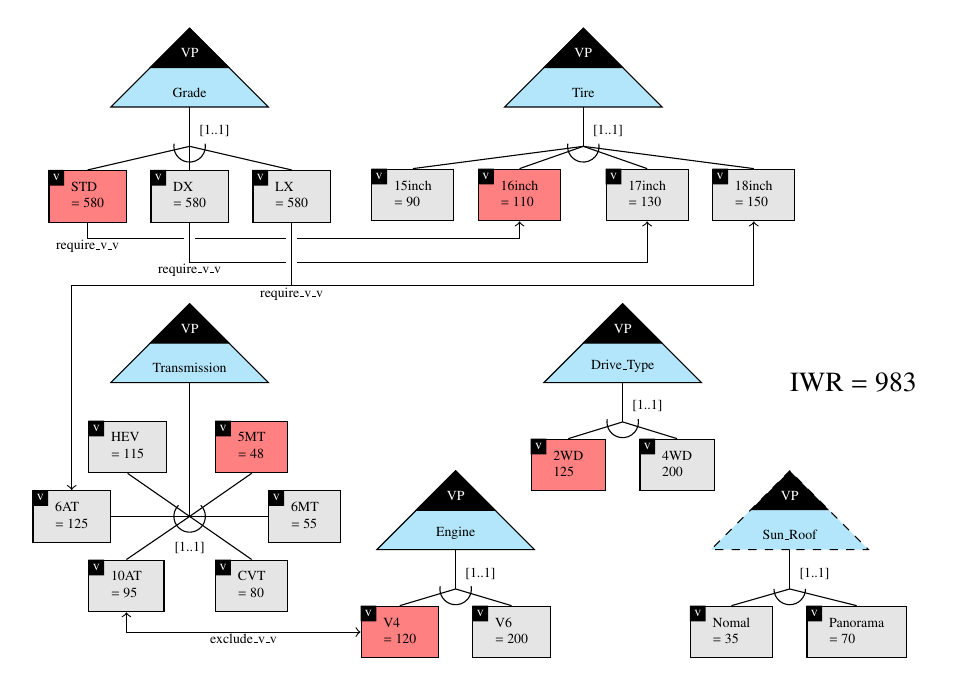
\begin{tikzpicture}
 % Grade
  \nodeVP{grade}{at={(0,0)}}{Grade};
  \nodeV{dx}{below=0.3cm of via_grade}{DX}{= 580};
  \draw(via_grade)--(dx.north);
  \nodeVchoiced{std}{left=0.3cm of dx}{STD}{= 580};
  \draw(via_grade)--(std.north);
  \nodeV{lx}{right=0.3cm of dx}{LX}{= 580};
  \draw(via_grade)--(lx.north);

  % Tire
  \nodeVP{tire}{right=5cm of grade}{Tire};
  \nodeVchoiced{16inch}{below left=0.4cm of via_tire}{16inch}{= 110};
  \nodeV{17inch}{below right=0.4cm of via_tire}{17inch}{= 130};
  \nodeV{15inch}{left=0.3cm of 16inch}{15inch}{= 90};
  \nodeV{18inch}{right=0.3cm of 17inch}{18inch}{= 150};
  \draw (via_tire)--(15inch.north);
  \draw (via_tire)--(16inch.north);
  \draw (via_tire)--(17inch.north);
  \draw (via_tire)--(18inch.north);

  % Transmission
  \nodeTrans{trans}{below=3.5cm of grade}{Transmission};
  \nodeV{6at}{left=1cm of via_trans}{6AT}{= 125};
  \nodeV{hev}{above right=0.3cm of 6at.north}{HEV}{= 115};
  \nodeV{10at}{below right=0.3cm of 6at.south}{10AT}{= 95};
  \nodeV{6mt}{right=1cm of via_trans}{6MT}{= 55};
  \nodeVchoiced{5mt}{above left=0.3cm of 6mt.north}{5MT}{= 48};
  \nodeV{cvt}{below left=0.3cm of 6mt.south}{CVT}{= 80};
  \draw (via_trans)--(10at.north);
  \draw (via_trans)--(6at.east);
  \draw (via_trans)--(hev.south);
  \draw (via_trans)--(6mt.west);
  \draw (via_trans)--(5mt.south);
  \draw (via_trans)--(cvt.north);

  % Drive_Type
  \nodeVP{drivetype}{right=5.5cm of trans}{Drive\_Type};
  \nodeVchoiced{2wd}{below left=0.3cm of via_drivetype}{2WD}{125};
  \draw (via_drivetype)--(2wd.north);
  \nodeV{4wd}{below right=0.3cm of via_drivetype}{4WD}{200};
  \draw (via_drivetype)--(4wd.north);


  % Sun_Roof
  \nodeVPdashed{sunroof}{below right=3cm of drivetype}{Sun\_Roof};
  \nodeV{nomal}{below left=0.3cm of via_sunroof}{Nomal}{= 35};
  \draw (via_sunroof)--(nomal.north);
  \nodeV{panorama}{below right=0.3cm of via_sunroof}{Panorama}{= 70};
  \draw (via_sunroof)--(panorama.north);

  % Engine
  \nodeVP{engine}{below left=3cm of drivetype}{Engine};
  \nodeVchoiced{v4}{below left=0.3cm of via_engine}{V4}{= 120};
  \draw (via_engine)--(v4.north);
  \nodeV{v6}{below right=0.3cm of via_engine}{V6}{= 200};
  \draw (via_engine)--(v6.north);
  
 

  % require
  \draw[->] (std.south)--++(0,-0.2) node[below=-1mm] {\tiny{require\_v\_v}} -|(16inch.south);
  \draw[white,line width=4pt](dx.south) ++(0,-0.1)--++(0,-0.5);
  \draw[->] (dx.south)--++(0,-0.5) node[below=-1mm] {\tiny{require\_v\_v}} -|(17inch.south);
  \draw[white,line width=4pt] (lx.south) ++(0,-0.1)--++(0,-0.8);
  \draw[->] (lx.south)--++(0,-0.8) node[below=-1mm] {\tiny{require\_v\_v}} -|(18inch.south);
  \draw[->] (lx.south)--++(0,-0.8) -|(6at.north);

  % exclude
  \draw[<->] (v4.west)-|(10at.south) node[pos=0.25,below=-1mm]{\tiny{exclude\_v\_v}};
  \node [right=2cm of drivetype] (iwr) {IWR = 983};
 \end{tikzpicture}

 
\end{frame}
%%%%%%%%%%%%%%%%%%%%%%%%%%%%%%%%%%%%%%%%%%%%%%%%%%%%
\begin{frame}{燃費制約 (CAFE基準)と目的関数}
\footnotesize
\begin{alertblock}{}
  \begin{itemize}\compress
  \item 装備仕様$g$の燃費を$FE_{g}$, 予想販売台数を$SV_{g}$,CAFE基準
    値を$X$とする.
    \[ 
      \frac{FE_{1}\cdot SV_1 + FE_{2} \cdot SV_2 + FE_{3} \cdot SV_3 }{SV_1 + SV_2 + SV_3}
      \geq X
      \qquad\qquad
      SV_1 + SV_2 + SV_3\longrightarrow \textrm{最大}
    \]
  \item $FE_{g}$と$SV_{g}$は,装備仕様$g$の\structure{\bf IWR値の和}か
    ら算出される.
  \end{itemize}

\end{alertblock}
% \begin{exampleblock}{}\centering
%   \renewcommand{\arraystretch}{0.9}
%   \begin{tabular}{l|l|r|c|c|c} %\cline{1-6}
%     \lw{装備タイプ}& \lw{装備オプション}& \lw{IWR値}& \multicolumn{3}{c}{装備仕様} \\\cline{4-6}
%                 &		&	& 1	& 2	& 3	\\\cline{1-6}
%     グレード 	&STD 		& 700	& \OK	&	&	\\%\cline{2-6}
%                 & DX 		& 700	&	& \OK	&	\\%\cline{2-6}	
%                 & LX 		& 700	& 	&	& \OK	\\\cline{1-6}
%     エンジン	& V4 		& 120	&	&	& \OK	\\%\cline{2-6}
%                 & V6 		& 200	& \OK	& \OK	& \\\cline{1-6}
%     タイヤ	& 16インチ	& 110	&  \OK	&	&	\\%\cline{2-6}
%                 & 17インチ 	& 130	&	& \OK	&	\\%\cline{2-6}
%                 & 18インチ 	& 150	& &	& \OK	\\\cline{1-6}
%     トランス	& MT		& 55	&	 &  &	\\%\cline{2-6}
%     ミッション	& HEV 	& 95	& \OK	& \OK	&	\\%\cline{2-6}
%                 & AT 		& 115	&	& 	& \OK \\\cline{1-6}
%     \multicolumn{1}{l}{} & \multicolumn{2}{r}{\structure{\bf IWR値の和}} & \multicolumn{1}{c}{1,105} &%
% 		\multicolumn{1}{c}{1,125} & \multicolumn{1}{c}{1,085}\\ 
% 	\end{tabular}
% \end{exampleblock}
\end{frame}
%%%%%%%%%%%%%%%%%%%%%%%%%%%%%%%%%%%%%%%%%%%%%%%%%%%%
\begin{frame}{最適解の例}
\begin{itemize}
 \item 装備仕様の数 G=3 (GradeはそれぞれSTD,DX,LXになるように設定)
 \item CAFE基準値 X=9.0
      
\end{itemize}
\begin{exampleblock}{}\centering
  %\renewcommand{\arraystretch}{0.9}
  \begin{tabular}{l|c|c|c} 
    \lw{装備}      & \multicolumn{3}{c}{装備仕様} \\ \cline{2-4}
                 & 1	& 2 	 & 3	\\  \hline
    Grade	 & STD	& DX	 & LX	\\
    Drive\_Type  & 2WD  & 2WD    & 2WD  \\
    Engine	 & V4	& V6	 & V6	\\
    Tire	 & 16	& 17	 & 18	\\
    Transmission & 5MT	& 6MT    & 10AT	\\
    Sun\_Roof    & -    & normal & -    \\ \hline
    IWR          & 983  & 1125   & 1180 \\ %\hline
    燃費(km/L)    & 10.2  & 8.9     & 8.5 \\ %\hline
    予想販売台数  & 745  & 1988   & 1171  \\ \hline
    平均燃費(km/L) & \multicolumn{3}{c}{\bf{9.0}} \\ 
    合計販売台数  & \multicolumn{3}{c}{\bf{3904}} \\
  \end{tabular}
\end{exampleblock}
 
\end{frame}
%%%%%%%%%%%%%%%%%%%%%%%%%%%%%%%%%%%%%%%%%%%%%%%%%%%%
\begin{frame}{解集合プログラミング(Answer Set Programing; ASP)}
 \begin{itemize}
 \item \structure{\bf ASP言語}は,一階論理に基づく知識表現言語の一種である.
 \item \structure{\bf ASPプログラム}は,ASPルールの有限集合である.
 \item \structure{\bf ASPシステム}は,安定モデル意味論~[Gelfond and Lifschitz '88]
   に基づく解集合を計算するシステムである.
 \item 近年,SAT技術を利用した高速なASPシステムが開発され,
%   ロボット工学,システム検証,システム生物学,
   スケジューリング,システム生物学
   など様々な分野への実用的応用が急速に拡大している.
 \end{itemize}
\vfill
 \begin{alertblock}{車両装備仕様問題に対してASPを用いる利点}
   \begin{itemize} 
   \item ASP言語の高い表現力により,各種制約を簡潔に記述できる.
   \item 高速なASPシステムを利用できる.
     \begin{itemize}
     \item 一階ASPプログラムを命題ASPプログラムに\alert{\bf 基礎化}した後,
       解集合を求めるシステムが主流
     \end{itemize}
   \item 解の最適性を保証できる.最適解の列挙も可能である.
   \end{itemize}
 \end{alertblock}
\end{frame}
%%%%%%%%%%%%%%%%%%%%%%%%%%%%%%%%%%%%%%%%%%%%%%%%%%%%
\begin{frame}{研究目的}
  \begin{alertblock}{目的}
    ASP技術を活用して,大規模な車両装備仕様問題を効率よく解くシステム
    を実現すること.
  \end{alertblock}
  \begin{block}{既存研究}
   \begin{itemize}
    \item CAFE問題に対するASP符号化(基本符号化と呼ぶ)
    \item Babieca・神戸大学・名古屋大学 共同研究(2019)
   \end{itemize}
  \end{block}
  \begin{block}{研究内容}
    \begin{enumerate}
     \item \structure{\bf 改良符号化を提案}
	   \begin{itemize}
	    \item 基本符号化での問題点
	    \item \alert{\bf IWR値の和の上下限を厳密に計算する}ように改良
	    % 	\item この改良により,基礎化後のルール数を少なく抑えることができ,
	    % 		大規模な問題に対する有効性が期待できる.
	   \end{itemize}
     \item \structure{\bf オプション数最小化}
	   \begin{itemize}
	    \item 販売台数の等しい複数の最適解に優劣をつけることが目的
	    \item コスト削減が見込める
	   \end{itemize}
	   
     \item \structure{\bf 排他制約への対応}
    \end{enumerate}
  \end{block}
  % \pause
  % \begin{itemize}
  % 	\item IWR値の和を表す制約モデルを用いて,2種類の提案符号化の違いを説明する.
  % \end{itemize}
\end{frame}
%%%%%%%%%%%%%%%%%%%%%%%%%%%%%%%%%%%%%%%%%%%%%%%%%%%% 
\begin{frame}{提案する車両装備ソルバーの概要}
 \begin{tikzpicture}
 \node [draw] (const) at (0,1) {制約・目的関数};
 \node [draw] (ins) at (0,0) {インスタンス};
 \node [draw] (fe) at (0,-1) {燃費テーブル};
 \node [draw] (sv) at (0,-2) {販売台数テーブル};
 \node [draw,inner sep=10pt] (asp) at (8,-1) {ASPプログラム};
 \node [draw,inner sep=10pt] (answerset) at (8,-5) {解集合};
 \node [draw,inner sep=10pt] (vd) at (0,-5) {装備仕様};

 \draw (ins)-|(2,-1);
 \draw [->] (fe)--(asp) node[pos=0.6,anchor=north]{\scriptsize{ASPファクト形式に変換}}; 
 \draw (sv)-|(2,-1);
 \draw [->] (const)-|(asp) node[pos=0.25,anchor=north]{\scriptsize{ASP符号化}};
 \draw [->] (asp)--(answerset) node[pos=0.5,anchor=west]{\scriptsize{ASPシステム}};
 \draw [->] (answerset)--(vd) node[pos=0.5,anchor=north]{\scriptsize{解釈}};
\end{tikzpicture}
\end{frame}
%%%%%%%%%%%%%%%%%%%%%%%%%%%%%%%%%%%%%%%%%%%%%%%%%%%% 
\begin{frame}[fragile]{CAFE問題のASPファクト形式}
 \begin{multicols}{2}
  \lstinputlisting[language={prolog}]{code/ovm.lp} 
 \end{multicols}
\end{frame}
%%%%%%%%%%%%%%%%%%%%%%%%%%%%%%%%%%%%%%%%%%%%%%%%%%%% 
\begin{frame}{基本符号化}
  \lstinputlisting[language={prolog}]{code/basic1.lp}
\end{frame}
%%%%%%%%%%%%%%%%%%%%%%%%%%%%%%%%%%%%%%%%%%%%%%%%%%%% 
\begin{frame}{基本符号化の問題点}
 
\end{frame}
%%%%%%%%%%%%%%%%%%%%%%%%%%%%%%%%%%%%%%%%%%%%%%%%%%%% 
\begin{frame}{改良符号化}
  \lstinputlisting[language={prolog}]{code/basic2.lp}
\end{frame}
%%%%%%%%%%%%%%%%%%%%%%%%%%%%%%%%%%%%%%%%%%%%%%%%%%%% 
\begin{frame}{実験1}
 考案したASP符号化の有効性を評価するために実験を行なった.
 \begin{itemize}
  \item ベンチマーク問題(計15問)
	\begin{itemize}
	 \item 企業から提供された問題(3問)に対して
	 \item 5通りのCAFE基準値$X \in \{8.5, 9.0, 9.5, 10.0, 10.5km/L\}$で生成
	 \item 求める装備仕様の数$G = 3$
	\end{itemize}
	\begin{exampleblock}\small
	 \centering
	 \begin{tabular}{ l|r r r }
	  問題		& 装備タイプ数	& 装備オプション数& 要求制約数 	\\ \hline
	  small	& 8			& 21		& 4		\\
	  medium	& 86		& 226		& 147	\\
	  big		& 315		& 1,337		& 0		\\
	 \end{tabular}
	\end{exampleblock}
  \item ASPシステム: \textit{clingo-5.4.0}
  \item 制限時間: 1問あたり2時間
  \item 実験環境: Mac mini, 3.2GHz, 64GB メモリ
 \end{itemize}
\end{frame}
%%%%%%%%%%%%%%%%%%%%%%%%%%%%%%%%%%%%%%%%%%%%%%%%%%%%
\begin{frame}{実験結果: 得られた最適値と最良値}
 \begin{exampleblock}{}
  \centering
  \scriptsize
  \begin{tabular}{l|r|r|r}
   \lw{問題} & \lw{CAFE基準値} & \multicolumn{2}{c}{販売台数} \\ \cline{3-4}
            &                 & 基本符号化 & 改良符号化 \\\hline    
   small & 8.5   & \alert{6,021*} & \alert{6,021*}       \\
   small & 9.0   & \alert{5,007*} & \alert{5,007*}       \\
   small & 9.5   & \alert{2,688*} & \alert{2,688*}       \\
   small & 10.0  & \alert{1,318*} & \alert{1,318*}       \\
   small & 10.5  & UNSAT          & UNSAT    \\\hline
   medium & 8.5  & 6,010          & \alert{6,021}        \\
   medium & 9.0  & \alert{5,595}  & \alert{5,595}        \\
   medium & 9.5  & \alert{3,447}  & 3,430        \\
   medium & 10.0 & 2,245          & \alert{2,250}        \\
   medium & 10.5 & 1,690          & \alert{1,845}        \\\hline
   big & 8.5     & TO             & \alert{3,877}        \\
   big & 9.0     & 1,038          & \alert{4,623}        \\
   big & 9.5     & 688            & \alert{3,121}        \\
   big & 10.0    & 1,634          & \alert{2,064}        \\
   big & 10.5    & 538            & \alert{904}         \\\hline
   \multicolumn{2}{l}{最適値・最良値の数} & \multicolumn{1}{r}{6} & \alert{13} \\
  \end{tabular}
 \end{exampleblock}
 \begin{itemize}
  \item 改良符号化は,基本符号化と比較して,多くの問題に対してより良い解を得た.
  \item 大規模な問題に対する改良符号化の優位性が確認できた.
 \end{itemize}	
\end{frame}
%%%%%%%%%%%%%%%%%%%%%%%%%%%%%%%%%%%%%%%%%%%%%%%%%%%%
\begin{frame}{実験2}
 グループ数を大きくして比較を行った.
 \begin{itemize}
  \item ベンチマーク問題
	\begin{itemize}
	 \item 小規模な問題(small)に対して
	 \item 5通りのCAFE基準値$X \in \{8.5, 9.0, 9.5, 10.0, 10.5km/L\}$
	 \item 3通りの装備仕様の数$G=3,6,12$で生成
	 \item 要求制約を追加
	\end{itemize}
  \item ASPシステム: \textit{clingo-5.4.0}
  \item 制限時間: 1問あたり1時間
  \item 実験環境: Mac mini, 3.2GHz, 64GB メモリ
 \end{itemize}
\end{frame}
%%%%%%%%%%%%%%%%%%%%%%%%%%%%%%%%%%%%%%%%%%%%%%%%%%%%
\begin{frame}{実験結果}
 % \begin{exampleblock}{}
 %  \centering
 %  \scriptsize
 %  \begin{tabular}{r|r|r|r}
 %   \lw{グループ数} & \lw{CAFE基準値} & \multicolumn{2}{c}{販売台数} \\ \cline{3-4}
 %             &                & 基本符号化 & 改良符号化 \\\hline    
 %   3 & 8.5   & \alert{6,021*} & \alert{6,021*}       \\
 %   3 & 9.0   & \alert{5,007*} & \alert{5,007*}       \\
 %   3 & 9.5   & \alert{2,688*} & \alert{2,688*}       \\
 %   3 & 10.0  & \alert{1,318*} & \alert{1,318*}       \\
 %   3 & 10.5  & UNSAT          & UNSAT    \\\hline
 %   6 & 8.5  & 6,010          & \alert{6,021}        \\
 %   6 & 9.0  & \alert{5,595}  & \alert{5,595}        \\
 %   6 & 9.5  & \alert{3,447}  & 3,430        \\
 %   6 & 10.0 & 2,245          & \alert{2,250}        \\
 %   6 & 10.5 & 1,690          & \alert{1,845}        \\\hline
 %   12 & 8.5     & TO             & \alert{3,877}        \\
 %   12 & 9.0     & 1,038          & \alert{4,623}        \\
 %   12 & 9.5     & 688            & \alert{3,121}        \\
 %   12 & 10.0    & 1,634          & \alert{2,064}        \\
 %   12 & 10.5    & 538            & \alert{904}         \\\hline
 %   \multicolumn{2}{l}{最適値・最良値の数} & \multicolumn{1}{r}{6} & \alert{13} \\
 %  \end{tabular}
 % \end{exampleblock}
 
\end{frame}
%%%%%%%%%%%%%%%%%%%%%%%%%%%%%%%%%%%%%%%%%%%%%%%%%%%%
\begin{frame}{オプション数最小化}
 \begin{block}{}
  \begin{itemize}
   \item インスタンスによっては最適解が複数得られる
   \item 
	 
  \end{itemize}
 \end{block}
 \begin{exampleblock}{}
  \centering
  \tiny
  \begin{tabular}{l|c|c|c||c|c|c||c|c|c} 
    \lw{装備}     & \multicolumn{3}{c||}{解1} & \multicolumn{3}{c||}{解2} & \multicolumn{3}{c}{解3}\\ \cline{2-10}
                 & STD	& DX 	 & LX	   & STD & DX  & LX    & STD & DX  & LX       \\  \hline
    Drive\_Type  & 4WD  & 2WD    & 4WD     & 2WD & 2WD & 4WD   & 2WD & 2WD & 4WD     \\
    Engine	 & V4	& V6	 & V6	   & V6  & V6  & V6    & V6  & V6  & V6      \\ 
    Tire	 & 16	& 17	 & 18	   & 16  & 17  & 18    & 16  & 17  & 18     \\
    Transmission & 5MT	& HEV    & 10AT	   & CVT & HEV & 10AT  & 6AT & HEV & 10AT     \\
    Sun\_Roof    & Panorama& -   & -       & Nomal& -  & -     & -   & -   & -       \\ \hline
    IWR          & 1128 & 1130   & 1255    & 1130 & 1130&1255  & 1130& 1130& 1255     \\ %\hline
    燃費(km/L)    & 8.9 & 8.8    & 8.0     & 8.8 & 8.8  & 8.0 & 8.8  & 8.8  & 8.0         \\ %\hline
    予想販売台数  & 2007  & 2007   & 1511   & 2007 & 2007 & 1511 & 2007& 2007& 1511       \\ \hline
    平均燃費(km/L) & \multicolumn{3}{c||}{\bf{8.6}} & \multicolumn{3}{c||}{\bf{8.5}} & \multicolumn{3}{c}{\bf{8.5}}\\ 
    合計販売台数  & \multicolumn{3}{c||}{\bf{5525}} & \multicolumn{3}{c||}{\bf{5525}}  &\multicolumn{3}{c}{\bf{5525}}\\
    オプション数  & \multicolumn{3}{c||}{\alert{14}} & \multicolumn{3}{c||}{\alert{13}}  &\multicolumn{3}{c}{\alert{12}}\\
  \end{tabular}
 \end{exampleblock}
 \begin{alertblock}{提案}
  最適解の中で優劣をつけるために目的関数として,オプション数の最小化を追加
 \end{alertblock}
\end{frame}
%%%%%%%%%%%%%%%%%%%%%%%%%%%%%%%%%%%%%%%%%%%%%%%%%%%%
\begin{frame}{オプション数最小化の実装例}
\begin{block}{}
 \begin{itemize}
  \item 選択された装備オプションの種類をカウントし,最小化する.
  \item 優先度を販売台数最大化の次にする.
 \end{itemize}
\end{block}
  \lstinputlisting[language={prolog}]{code/obj_op.lp}
\end{frame}
%%%%%%%%%%%%%%%%%%%%%%%%%%%%%%%%%%%%%%%%%%%%%%%%%%%%
% \begin{frame}{最適解の個数}
%  \begin{itemize}
%   \item clingoはオプションを加えることで最適解の列挙が可能
%   \item 改良符号化を用いて,問題smallに対して最適解の個数を調査
%  \end{itemize}

%  \begin{exampleblock}{}\centering
%   \begin{tabular}{l|r|r|c}
%    問題 & CAFE基準値 & 販売台数 & 最適解の個数 \\ \hline
%    small & 8.5   & 6,021 & \alert{2} \\ 
%    small & 9.0   & 5,007 & \alert{2} \\
%    small & 9.5   & 2,688 & 1 \\
%    small & 10.0  & 1,318 & 1 \\
%    small & 10.5  & UNSAT & - \\ 
%   \end{tabular}
%  \end{exampleblock}
%  \begin{itemize}
%   \item CAFE基準値が8.5,9.0km/Lのとき,最適解が複数存在 
%   \item 最適解の中でもより優れた解を選択したい
%  \end{itemize}

%  \begin{alertblock}{提案}
%   目的関数として,オプション数の最小化を追加
%  \end{alertblock}
% \end{frame}
% %%%%%%%%%%%%%%%%%%%%%%%%%%%%%%%%%%%%%%%%%%%%%%%%%%%%% 
% \begin{frame}{共通部品数の最大化}
%  \begin{exampleblock}{}\centering
%   \small
%   \begin{tabular}{l|l|r|c|c|c} %\cline{1-6}
%     \lw{装備タイプ}& \lw{装備オプション}	& \lw{IWR値}& \multicolumn{3}{c}{装備仕様} \\\cline{4-6}
%                 &			&		& 1	& 2	& 3	\\\cline{1-6}
%     グレード 	& \alert{STD}		& 700	& \OK	&	&	\\%\cline{2-6}
%                 & \alert{DX}		& 700	&	& \OK	&	\\%\cline{2-6}	
%                 & \alert{LX}		& 700	& 	&	& \OK	\\\cline{1-6}
%     エンジン	& \alert{V4} 			& 120	&	&	& \OK	\\%\cline{2-6}
%                 & \alert{V6} 			& 200	& \OK	& \OK	& \\\cline{1-6}
%     タイヤ	& \alert{16インチ}	& 110	&  \OK	&	&	\\%\cline{2-6}
%                 & \alert{17インチ} 	& 130	&	& \OK	&	\\%\cline{2-6}
%                 & \alert{18インチ} 	& 150	& &	& \OK	\\\cline{1-6}
%     トランス	& MT		& 55	&	 &  &	\\%\cline{2-6}
%     ミッション	& \alert{HEV} 	& 95	& \OK	& \OK	&	\\%\cline{2-6}
%                 & \alert{AT} 		& 115	&	& 	& \OK \\\cline{1-6}
%     \multicolumn{1}{c}{選択オプション数} & \multicolumn{1}{l}{\alert{10}} & \multicolumn{4}{r}

%   \end{tabular}
%  \end{exampleblock}

%  \begin{alertblock}{提案手法}
%   選択される装備オプションの数を最小化する.
%  \end{alertblock}
% \end{frame}
% %%%%%%%%%%%%%%%%%%%%%%%%%%%%%%%%%%%%%%%%%%%%%%%%%%%%% 
\begin{frame}{オプション数最小化}
 \begin{block}{実験概要}
  \begin{itemize}
   \item オプション数最小化の有無で最適解の個数を比較
   \item インスタンスはOVMで示したCAFE問題の例を使用
  \end{itemize}
 \end{block}
 
 \begin{exampleblock}{実験結果}\centering
  \begin{tabular}{l|r|r|c|c}
   \lw{問題} & \lw{CAFE基準値} & \lw{販売台数} & \multicolumn{2}{c}{最適解の個数} \\ \cline{4-5}
            &                &              & 改良符号化 & +共通部品数最大化 \\ \hline        
   small & 8.5   & 5,525 & 3 & 1\\ 
   small & 9.0   & 3,904 & 2 & 2 \\
   small & 9.5   & 1,699 & 1 & 1 \\
   small & 10.0  & UNSAT & - & - \\
   small & 10.5  & UNSAT & - & - \\ 
  \end{tabular}
 \end{exampleblock}
 \begin{itemize}
  \item CAFE基準値8.5km/Lでは,最適解の個数が減少した
  \item CAFE基準値9.0km/Lでは,最適解が複数のままだった
 \end{itemize}
\end{frame}
%%%%%%%%%%%%%%%%%%%%%%%%%%%%%%%%%%%%%%%%%%%%%%%%%%%%% 
\begin{frame}{まとめ}
 \begin{itemize}
  \item \structure{\bf 車両装備仕様問題に対する2種類のASP符号化を考案}
	\begin{itemize}
	 \item 問題を簡潔に記述できることを確認した
	       (ASPのルール\alert{\bf 11}個).
	 \item 改良符号化は,基本符号化と比較して,
	       \alert{\bf IWR値の和の上下限を厳密に計算する}ように改良されている.
	\end{itemize}
  \item \structure{\bf 企業から提供された実データを用いた実験・評価}
	\begin{itemize}
	 \item 小規模な問題に対して,その最適解を得ることができた.
	 \item 大規模な問題に対して,改良符号化の優位性が確認できた.
	\end{itemize}
 \end{itemize}
 \vfill
 \begin{alertblock}{今後の課題}
  \begin{itemize}
   \item 企業の技術者へのヒアリングに基づく問題拡張
	 \begin{itemize}
	  \item 装備オプション間の排他制約などの新たな制約の追加
	  \item 共通部品の最大化などの新たな目的関数の追加
	 \end{itemize}
  \end{itemize}
 \end{alertblock}
\end{frame}
%%%%%%%%%%%%%%%%%%%%%%%%%%%%%%%%%%%%%%%%%%%%%%%%%%%%% 


%%%%%%%%%%%%%%%%%%%%%%%%%%%%%%%%%%%%%%%%%%%%%%%%%%%% 
% \begin{frame}
% \frametitle{ASPを用いた問題解法}

% \begin{center}%\small
% \begin{tikzpicture}[
%   ->,>=stealth',shorten >=1pt,auto,node distance=1cm,
%   rectangle/.style = {
%     draw,thick,fill=red!10,rounded corners=2pt,
%     minimum width=3cm,minimum height=1.0cm}
%   ]
%   \node[rectangle] (n1) {車両装備仕様問題};
%   \node[rectangle] (n2) [right=3cm of n1] {ASPプログラム};
%   \path[->,draw,line width=1pt] (n1) edge node {モデリング} (n2);
%   \node[rectangle] (n3) [below=1cm of n2] {解集合};
%   \path[->,draw,line width=1pt] (n2) edge node {ASPシステム} (n3);
%   \node[rectangle] (n4) [below=1cm of n1] {問題の解};
%   \path[->,draw,line width=1pt] (n3) edge node {解釈} (n4);
%   \path[->,draw,dashed,line width=1pt] (n1) edge node {} (n4);
% %  \only<2>{\draw[line width=1.2pt,color=red,dashed] (4,1) -- (8,1) -- (8,-1) -- (4,-1) -- cycle;}
% %  \only<3>{\draw[line width=1.2pt,color=red,dashed] (4,1) -- (8,1) -- (8,-3) -- (4,-3) -- cycle;}
% %  \only<4>{\draw[line width=1.2pt,color=red,dashed] (-2,-1) -- (8,-1) -- (8,-3) -- (-2,-3) -- cycle;}
% \end{tikzpicture}
% \end{center}
% \begin{enumerate}
% \item 問題を\structure{ASPプログラム}としてモデリングする.
% \item ASPシステムは,一階ASPプログラムを命題ASPプログラムに基礎化した後,
%   \structure{解集合}(一種の最小モデル)を計算する.
% \item 解集合を解釈して元の問題の解を得る.
% \end{enumerate}

% \end{frame}
%%%%%%%%%%%%%%%%%%%%%%%%%%%%%%%%%%%%%%%%%%%%%%%%%%%%
\begin{frame}{基本符号化のベースとなる制約モデル}
  \begin{block}{問題の入力 (一部)}
    \begin{itemize}\compress
     \item $V$: 装備オプションの集合
     \item $w_{j}$: 装備オプション$j\in V$のIWR値
     \item $G$: 求めたい装備仕様の数
    \end{itemize}
  \end{block}

  \begin{block}{IWR値の和に関する制約}
  \[
    \begin{array}{lr}
      x_{jg}\in\{0,1\} & j\in V, g\in\{1,\ldots,G\} \\
      y_{g}\in\{0,\ldots, \displaystyle\sum_{j\in V}w_{j}\} & g\in\{1,\ldots,G\} \\
      y_{g} = \displaystyle\sum_{j\in V}w_{j}x_{jg} & g\in\{1,\ldots,G\}
    \end{array}
  \]
  \end{block}

  \begin{itemize}\small
  \item 0-1変数$x_{jg}$は,装備オプション$j$が装備仕様$g$で選択されることを意味
  \item 整数変数$y_{g}$は,装備仕様$g$のIWR値の和を表す.
  \end{itemize}
\end{frame}
%%%%%%%%%%%%%%%%%%%%%%%%%%%%%%%%%%%%%%%%%%%%%%%%%%%%
\begin{frame}{改良符号化での制約モデル}
  \begin{alertblock}{}
      必須装備タイプと個数制約の性質を利用して,
      IWR 値の和($y_g$)の上下限を厳密に計算することができる.
  \end{alertblock}

  \begin{block}{問題の入力 (一部)}
    \begin{itemize}\compress
    % \item $V$: 装備オプションの集合
    % \item $w_{j}$: 装備オプション$j\in V$のIWR値
    % \item $G$: 求めたい装備仕様の数
    \item $VP$: 装備タイプの集合
    \item $VP^{*}\subseteq VP$: 必須装備タイプの集合
    \item $V_{i}\subseteq V$: 装備タイプ$i\in VP$が選択できる装備オプションの集合
    \end{itemize}
  \end{block}

  \begin{block}{IWR値の和に関する制約}
  \[
    \begin{array}{lr}
      x_{jg}\in\{0,1\} & j\in V, g\in\{1,\ldots,G\} \\
      \alert{y_{g}\in\{\displaystyle\sum_{i\in VP^{*}}\min_{j\in
      V_{i}}w_{j},\ldots, \sum_{i\in VP}\max_{j\in V_{i}}w_{j}\}} 
      & g\in\{1,\ldots,G\} \\
      y_{g} = \displaystyle\sum_{j\in V}w_{j}x_{jg} & g\in\{1,\ldots,G\}
    \end{array}
  \]
  \end{block}
\end{frame}
% %%%%%%%%%%%%%%%%%%%%%%%%%%%%%%%%%%%%%%%%%%%%%%%%%%%% 
% \begin{frame}{IWR値の和}

%   \begin{itemize}
%   \item $G$: 求めたい装備仕様の数
%   \item $V$: 装備オプションの集合
%   \item $w_{j}$: 装備オプション$j\in V$のIWR値
%   \end{itemize}
%   \begin{itemize}
%   \item $x_{jg}$: 装備オプション$j\in V$が装備仕様$g\in\{1,\ldots,G\}$で選択されることを意味
%     する0-1変数
%   \item $y_{g}$: 装備仕様$g\in\{1,\ldots,G\}$のIWR値の和を表す整数変数
%   \end{itemize}
%   \[
%     x_{jg}\in\{0,1\} \qquad
%     y_{g}\in\{0,\ldots, \sum_{j\in V}w_{j}\} \qquad
%     y_{g} = \sum_{j\in V}w_{j}x_{jg}
%   \]

%   \[
%     x_{jg}\in\{0,1\} \qquad
%     y_{g}\in\{\sum_{i\in VP}\min_{j\in V_{i}}w_{j},\ldots, \sum_{i\in VP}\max_{j\in V_{i}}w_{j}\} \qquad
%     y_{g} = \sum_{j\in V}w_{j}x_{jg}
%   \]
% \end{frame}
%%%%%%%%%%%%%%%%%%%%%%%%%%%%%%%%%%%%%%%%%%%%%%%%%%%%
\appendix
%%%%%%%%%%%%%%%%%%%%%%%%%%%%%%%%%%%%%%%%%%%%%%%%%%%%
\begin{frame}{要求制約}
 \begin{alertblock}{}
  要求制約$X\longrightarrow Y$は,装備オプション$X$が選択されるならば,
  装備オプション$Y$も選択されなければならないことを意味する.
 \end{alertblock}
 \begin{center}
  STD$\longrightarrow$16インチ,\quad
  DX$\longrightarrow$17インチ,\quad
  LX$\longrightarrow$18インチ,\quad
  LX$\longrightarrow$AT
 \end{center}
 \begin{exampleblock}{}\small
  \centering
  \begin{tabular}{l|l|r|c|c|c} %\cline{1-6}
   装備タイプ	& 装備オプション 	& IWR値	& \multicolumn{3}{c}{装備仕様} \\\cline{4-6}
                &		&	& 1	& 2	& 3	\\\cline{1-6}
   グレード 	& STD 		& 700	& \OK	&	&	\\\cline{2-6}
                & DX 		& 700	&	& \OK	&	\\\cline{2-6}	
                & LX 		& 700	& 	&	& \OK	\\\cline{1-6}
   エンジン	& V4 		& 120	&	&	& \OK	\\\cline{2-6}
                & V6 		& 200	& \OK	& \OK	& \\\cline{1-6}
   タイヤ	& 16インチ	& 110	&  \OK	&	&	\\\cline{2-6}
                & 17インチ 	& 130	&	& \OK	&	\\\cline{2-6}
                & 18インチ 	& 150	& &	& \OK	\\\cline{1-6}
   トランス	& MT		& 55	&	 &  &	\\\cline{2-6}
   ミッション	& HEV 	        & 95	& \OK	& \OK	&	\\\cline{2-6}
                & AT 		& 115	&	& 	& \OK %\\\cline{1-6}
  \end{tabular}
 \end{exampleblock}
\end{frame}
%%%%%%%%%%%%%%%%%%%%%%%%%%%%%%%%%%%%%%%%%%%%%%%%%%%%
\begin{tabular}{l|p{8cm}}
  符号化名 & 遷移制約 \\\hline
  origin & 任意の二つの頂点に対し違反する組合せを列挙することで表現  \\ \hline
  changed & 遷移制約を ASP の個数制約を用いて表現\\\hline
  unchanged & 「各遷移で色が変化しない頂点は$|V|-1$個」という制約を,
         ASPの個数制約を用いて表現
\end{tabular}
%%%%%%%%%%%%%%%%%%%%%%%%%%%%%%%%%%%%%%%%%%%%%%%%%%%%
\begin{frame}{比較結果: 基礎化後のルール数} 
 \begin{exampleblock}{IWR値の和に関する制約の基礎化後のルール数} \centering 
  \begin{tabular}{c|r|r|r}
   問題 	& 基本符号化 	& 改良符号化 & 削減率(\%)	\\\hline
   small 	& 2,820		& \alert{576} & 80\% $\downarrow$ \\
   medium 	& 7,545		& \alert{1,758} & 80\% $\downarrow$ \\
   big 		& 62,745	& \alert{1,488} & 98\% $\downarrow$ \\
  \end{tabular}
 \end{exampleblock}
 \begin{itemize}
  \item 改良符号化では,IWR値の和の上下限を厳密に計算することで,
	基礎化後のルール数が大幅に削減されることが確認できた.
 \end{itemize}
\end{frame}
%%%%%%%%%%%%%%%%%%%%%%%%%%%%%%%%%%%%%%%%%%%%%%%%%%%%
\begin{frame}{比較結果: CPU時間}
 最適解が求まった問題インスタンスでのCPU時間を比較する.
 \begin{exampleblock}{} \centering 
  \begin{tabular}{crrr}
   問題		& CAFE基準値(km/L)	 & 基本符号化(s)  & 改良符号化(s)   \\\hline
   small 	& 8.5  & 37.868          	& \alert{23.318}          \\
   small	& 9.0  & 48.965          & \alert{43.362}          \\
   small	& 9.5  & \alert{95.110}          & 173.172         \\
   small	& 10.0 & 99.954          & \alert{0.343}           \\
   small	& 10.5 & 439.613         & \alert{0.080}           \\\hline
   \multicolumn{2}{r}{平均}		 & 144.302			& \alert{48.055}
  \end{tabular}
 \end{exampleblock}
 \begin{itemize}
  \item 5問中4問に対して,改良符号化の方が高速に最適解を求めた.
  \item 平均では,改良符号化のCPU時間は基本符号化の約1/3であった.
 \end{itemize}
\end{frame}
%%%%%%%%%%%%%%%%%%%%%%%%%%%%%%%%%%%%%%%%%%%%%%%%%%%% 
\begin{frame}
 \frametitle{ASPを用いた問題解法}
 \begin{center}%\small
  \begin{tikzpicture}[
   ->,>=stealth',shorten >=1pt,auto,node distance=1cm,
   rectangle/.style = {
   draw,thick,fill=red!10,rounded corners=2pt,
   minimum width=3cm,minimum height=1.0cm}
   ]
   \node[rectangle] (n1) {車両装備仕様問題};
   \node[rectangle] (n2) [right=3cm of n1] {ASPプログラム};
   \path[->,draw,line width=1pt] (n1) edge node {モデリング} (n2);
   \node[rectangle] (n3) [below=1cm of n2] {解集合};
   \path[->,draw,line width=1pt] (n2) edge node {ASPシステム} (n3);
   \node[rectangle] (n4) [below=1cm of n1] {問題の解};
   \path[->,draw,line width=1pt] (n3) edge node {解釈} (n4);
   \path[->,draw,dashed,line width=1pt] (n1) edge node {} (n4);
   %  \only<2>{\draw[line width=1.2pt,color=red,dashed] (4,1) -- (8,1) -- (8,-1) -- (4,-1) -- cycle;}
   %  \only<3>{\draw[line width=1.2pt,color=red,dashed] (4,1) -- (8,1) -- (8,-3) -- (4,-3) -- cycle;}
   %  \only<4>{\draw[line width=1.2pt,color=red,dashed] (-2,-1) -- (8,-1) -- (8,-3) -- (-2,-3) -- cycle;}
  \end{tikzpicture}
 \end{center}
 \begin{enumerate}
  \item 問題を\structure{ASPプログラム}としてモデリングする.
  \item ASPシステムは,一階ASPプログラムを命題ASPプログラムに基礎化した後,
  \item 解集合を解釈して元の問題の解を得る.
	\structure{解集合}(一種の最小モデル)を計算する.
 \end{enumerate}

\end{frame}
%%%%%%%%%%%%%%%%%%%%%%%%%%%%%%%%%%%%%%%%%%%%%%%%%%%%
\begin{frame}{車両装備仕様問題の例}
\begin{exampleblock}{}\centering
  \begin{tabular}{l|l|r|c|c|c}
    \lw{装備タイプ}& \lw{装備オプション}& \lw{IWR値}& \multicolumn{3}{c}{装備仕様} \\\cline{4-6}
                &		&	& 1	& 2	& 3	\\\cline{1-6}
    グレード 	& STD 		& 700	& \onslide<2->{\OK}	&	&	\\%\cline{2-6}
                & DX 		& 700	&	& \onslide<2->{\OK}	&	\\%\cline{2-6}	
		& LX 		& 700	& 	&	& \onslide<2->{\OK}	\\\cline{1-6}
    エンジン	& V4 		& 120	&	&	& \onslide<2->{\OK}	\\%\cline{2-6}
                & V6 		& 200	& \onslide<2->{\OK}	& \onslide<2->{\OK}	& \\\cline{1-6}
    タイヤ	& 16インチ	& 110	& \onslide<2->{\OK}	&	&	\\%\cline{2-6}
		& 17インチ 	& 130	&	& \onslide<2->{\OK}	&	\\%\cline{2-6}
		& 18インチ 	& 150	&       &	& \onslide<2->{\OK}	\\\cline{1-6}
    トランス	& MT		& 55	&	& &	\\%\cline{2-6}
    ミッション	& HEV 	        & 95	&	\onslide<2->{\OK}& \onslide<2->{\OK}	&\\%\cline{2-6}
                & AT 		& 115	&	& 	& \onslide<2->{\OK}
  \end{tabular}
\end{exampleblock}
%
\begin{itemize}
\item \onslide<1->{装備タイプはすべて\structure{\bf 必須}とする.}
\item \onslide<2>{実行可能解の例を{\OK}マークで示す.}
\end{itemize}
\end{frame}
%%%%%%%%%%%%%%%%%%%%%%%%%%%%%%%%%%%%%%%%%%%%%%%%%%%%
\begin{frame}[shrink]{個数制約}
\begin{alertblock}{}
  各装備仕様$g$, 各装備タイプ$i$に対して,$i$が$g$で選択されるならば,
  $i$の装備オプションのうち,ちょうど1つが$g$で選択される.
\end{alertblock}
\begin{exampleblock}{}\centering
  \begin{tabular}{l|l|r|c|c|c} %\cline{1-6}
    \lw{装備タイプ}& \lw{装備オプション}	& \lw{IWR値}& \multicolumn{3}{c}{装備仕様} \\\cline{4-6}
                &			&		& 1	& 2	& 3	\\\cline{1-6}
    グレード 	&STD 			& 700	& \OK	&	&	\\%\cline{2-6}
                & DX 			& 700	&	& \OK	&	\\%\cline{2-6}	
                & LX 			& 700	& 	&	& \OK	\\\cline{1-6}
    エンジン	& V4 			& 120	&	&	& \OK	\\%\cline{2-6}
                & V6 			& 200	& \OK	& \OK	& \\\cline{1-6}
    タイヤ	& 16インチ	& 110	&  \OK	&	&	\\%\cline{2-6}
                & 17インチ 	& 130	&	& \OK	&	\\%\cline{2-6}
                & 18インチ 	& 150	& &	& \OK	\\\cline{1-6}
    トランス	& MT		& 55	&	 &  &	\\%\cline{2-6}
    ミッション	& HEV 	& 95	& \OK	& \OK	&	\\%\cline{2-6}
                & AT 		& 115	&	& 	& \OK %\\\cline{1-6}
  \end{tabular}
\end{exampleblock}
\end{frame}
%%%%%%%%%%%%%%%%%%%%%%%%%%%%%%%%%%%%%%%%%%%%%%%%%%%%

\end{document}
%%% Local Variables:
%%% mode: japanese-latex
%%% TeX-master: t
%%% End:
